\documentclass[a4paper,14pt]{article} % тип документа
%\documentclass[14pt]{extreport}
\usepackage{extsizes} % Возможность сделать 14-й шрифт


\usepackage{geometry} % Простой способ задавать поля
\geometry{top=25mm}
\geometry{bottom=35mm}
\geometry{left=20mm}
\geometry{right=20mm}

\setcounter{section}{0}

%%%Библиотеки
%\usepackage[warn]{mathtext}
%\usepackage[T2A]{fontenc} % кодировка
\usepackage[utf8]{inputenc} % кодировка исходного текста
\usepackage[english,russian]{babel} % локализация и переносы
\usepackage{caption}
\usepackage{listings}
\usepackage{amsmath,amsfonts,amssymb,amsthm,mathtools}
\usepackage{wasysym}
\usepackage{graphicx}%Вставка картинок правильная
\usepackage{float}%"Плавающие" картинки
\usepackage{wrapfig}%Обтекание фигур (таблиц, картинок и прочего)
\usepackage{fancyhdr} %загрузим пакет
\usepackage{lscape}
\usepackage{xcolor}
\usepackage{dsfont}
%\usepackage{indentfirst}
\usepackage[normalem]{ulem}
\usepackage{hyperref}




%%% DRAGON STUFF
\usepackage{scalerel}
\usepackage{mathtools}

\DeclareMathOperator*{\myint}{\ThisStyle{\rotatebox{25}{$\SavedStyle\!\int\!\!\!$}}}

\DeclareMathOperator*{\myoint}{\ThisStyle{\rotatebox{25}{$\SavedStyle\!\oint\!\!\!$}}}

\usepackage{scalerel}
\usepackage{graphicx}
%%% END 

%%%Конец библиотек

%%%Настройка ссылок
\hypersetup
{
colorlinks=true,
linkcolor=blue,
filecolor=magenta,
urlcolor=blue
}
%%%Конец настройки ссылок


%%%Настройка колонтитулы
	\pagestyle{fancy}
	\fancyhead{}
	\fancyhead[L]{Домашнее задание}
	\fancyhead[R]{Крейнин Матвей, группа Б05-005}
	\fancyfoot{}
    \fancyfoot[C]{\thepage}
    \fancyfoot[R]{ТРЯП}
%%%конец настройки колонтитулы



\begin{document}
%%%%Начало документа%%%%

\section{Задание 2}
\subsection{Задача 1}

$\textbf{1.}$ R = $(bb|b|\mathcal{E})$$(a^{+}(bb|b|\mathcal{E}))^{*}$
Теперь доказательство корректности регулярного выражения, пусть n = 1, для слова a, регулярное выражение считается корректно, в $(bb|b|\mathcal{E})$ будет $\mathcal{E}$
потом считается a из $a^{+}$ потом считается $\mathcal{E}$ и на этом закончится (для слова b получается почти аналогично), для aa, ab, bb, ba - всё очевидно, в первом случае считается две буквы а из второго скобки, для ab считается a потом b из второй скобки, для bb считается две буквы b из первой скобки, для ba считается буква b из первой скобки, потом буква a из второй.
База доказана

Предположим, что это верно для слова длины n, тогда рассмотрим слово длины n+1.
n > 2. Тогда получается, что первая скобка считалась. У нас слово длины n при добавлении буквы а может оканчиваться на любую букву, считывание произойдёт, т.к. во второй скобке считается просто еще одна буква a.
В случае же приписывании буквы b слово длины n может оканчиваться на букву a, либо на одну b. В случае буквы a считается эта буква во второй скобке, в случае b произойдет считывание двух букв b, вместо одной буквы b.
Т.к. до этого по индукции было предположено, что трех одинаковых подряд идущих букв нет, то и в новом построенном слове такой буквы не будет. Если же слово длины n будет оканчиваться на две буквы bb и новая буква b, то РВ R его не считает, т.к. в указанном регулярном выражении не может быть трех букв b подряд, их разделяет хотя бы одна буква a.  

\subsection{Задача 2}
$\textbf{1.}$ Автомат $\mathcal{A}$: $Q = \{q_0, q_1, q_2\}$, $\Sigma = \{0, 1\}$, $q_0 = q_0$, F = $q_1$
\begin{tabular}{ | l | l | l | }
    \hline
    $\delta:$ & 0       & 1     \\ \hline
    $q_0$ & $q_0$   & $q_1$ \\
    $q_1$ & $q_2$   & $q_0$ \\
    $q_2$ & $q_1$   & $q_2$ \\
    \hline
    \end{tabular}

\vspace{10mm}

Автомат $\mathcal{B}$: $Q = \{q_0, q_1, q_2\}$, $\Sigma = \{0, 1\}$, $q_0 = q_0$, F = $q_1$
\begin{tabular}{ | l | l | l | }
    \hline
    $\delta:$ & 0       & 1             \\ \hline
    $q_0$ & $q_0$       & $q_1$         \\
    $q_1$ & $q_2, q_0$  & не определен  \\
    $q_2$ & $q_1$       & $q_2$         \\
    \hline
    \end{tabular}

\newpage
$\textbf{2.}$ Автомат $\mathcal{A}$ является детерменированным, это видно из таблицы переходов, т.к. там однозначно определен переход из каждого состояния в каждое.

Автомат $\mathcal{B}$ не является детерменированным, т.к. у него не определен однозначно переход из состояния $q_1$ по букве 0 (может быть $q_2$, а может быть $q_0$), переход по букве 1 вообще не определен.

$\textbf{3.}$ При старте автомат $\mathcal{A}$ находится в состоянии $q_0$. По букве 0 автомат останется в состоянии $q_0$, по букве 1 автомат перейдёт в состояние $q_1$, по букве 1 перейдёт обратно в состояние $q_0$,
по букве 0 и 0 останется в состоянии $q_0$, потом по букве 1 перейдёт в состоянии $q_1$. Состояние $q_1$ является принимающим состоянием, поэтому слово $\omega \in \mathcal{L(A)}.$

$\textbf{4.}$ При старте автомат $\mathcal{A}$ находится в состоянии $q_0$. При считывании буквы 0 автомат переходит в состояние $q_0$, потом при считывании буквы 1 автомат переходит в состояниие $q_1$.
При считывании буквы 0 поведение автомата не определено однозначно и нужно рассматривать два возможных варианта.

Первый вариант: автомат переходит в состояние $q_2$, при считывании буквы 1 автомат переходит в состояние $q_2$, при считывании буквы 0 переходит в состояние $q_1$. 
Дальнейшее поведение автомата не определено может переходить опять в два варианта (1.1 и 1.2).

1.1 вариант: автомат переходит в состояние $q_2$, потом считывает букву 1 и остаётся в состоянии $q_2$. Слово $\omega$ не считается считанным, т.к. автомат не пришел в принимающее состояние $q_1$.

1.2 вариант: автомат переходит в состояние $q_1$, потом считывает букву 1 и переходит в состояние $q_1$. Слово v считается считанным, т.к. автомат перешел в принимающее состояние $q_1$.

Второй вариант: автом переходит в состояние $q_1$, по букве 1 автомат переходит в состояние $q_1$. Потом возможно два варианта (2.1 и 2.2).

2.1: автомат переходит в состояние $q_2$, потом по букве 0 опять переходит в $q_1$, дальнейший переход по букве 1 не определен. Автомат может не принять слово v.

2.2: автомат переходит в состояние $q_1$, потом по букве 0 остается в состоянии $q_0$, по букве 1 переходит в состояние $q_1$. Автомат пришел в принимающее состояние, слово будет считано.

В общем случае слово v = 0101001 не будет распознано автоматом $\mathcal{B}$.

\textbf{5.} Слово, принадлежащее $\mathcal{L(A)}$, $\omega$ = 1. 

Слово, принадлежащее $\mathcal{L(B)}$, $\omega$ = 01

Слово, не принадлежащее $\mathcal{L(A)}$, $\omega$ = 010. 

Слово, не принадлежащее $\mathcal{L(B)}$, $\omega$ = 0.

\subsection{Задача 3}
$q_0$ - начальное состояние автомата, $q_3$ - принимающее состояние автомата.
Автомат переходит из состояния $q_0$ в $q_3$ только если встретится последовательность aab. В остальных случаях он не достигнет принимающего состояния $q_3$.

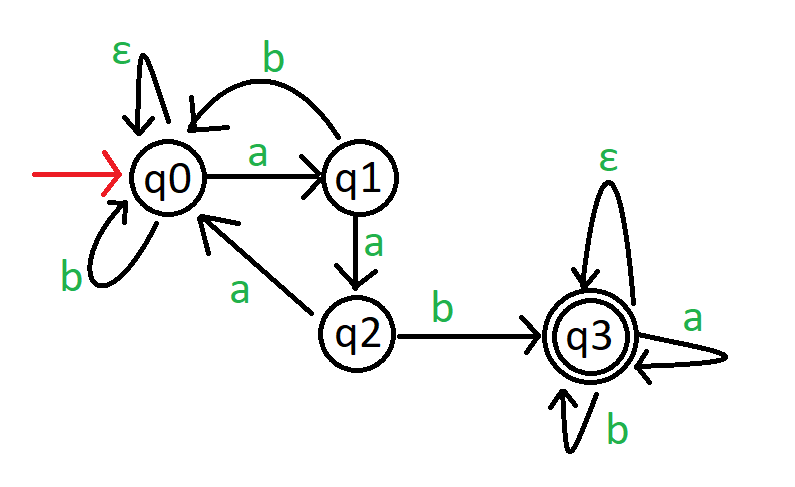
\includegraphics[scale=0.6]{01.png}

\subsection{Задача 4}
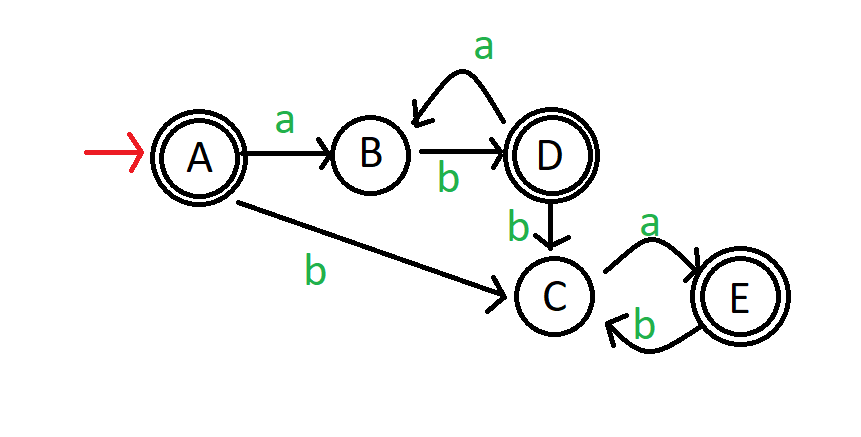
\includegraphics[scale=0.6]{02.png}

Да, регулярное выражение $(ab)^{*}(ba)^{*}$ порождает тот же язык, что распознает автомат M.

Но этот автомат не определен для пустого слова. И, просто подав на вход пустое слово, можно получить, что автомат не отработает это пустое слово, т.к. поведение для него в этом случае будет не определено, и в какое состояние он перейдёт непонятно из условий заданных в задаче.

Если считать, что пустое слово оставляет в том же состоянии, в котором он находится, то это регулярное выражение порождает тот же язык, что распознает автомат M.

Таблица получена по методу построения дерева из листьев (сделано в тетради).
\{1a, 3b, $5_{\triangleleft}$\} root $\{5_{\triangleleft}\}$

\vspace{5mm}
\begin{tabular}{ | l | l |}
    \hline
    i & followpos(i)     \\ \hline
    $1_a$ & $2_b$       \\
    $2_b$ & $1_a, 3_b, 5_{\triangleleft}$  \\
    $3_b$ & $4_a$       \\
    $4_a$ & $3_b, 5_{\triangleleft}$       \\
    \hline
    \end{tabular}


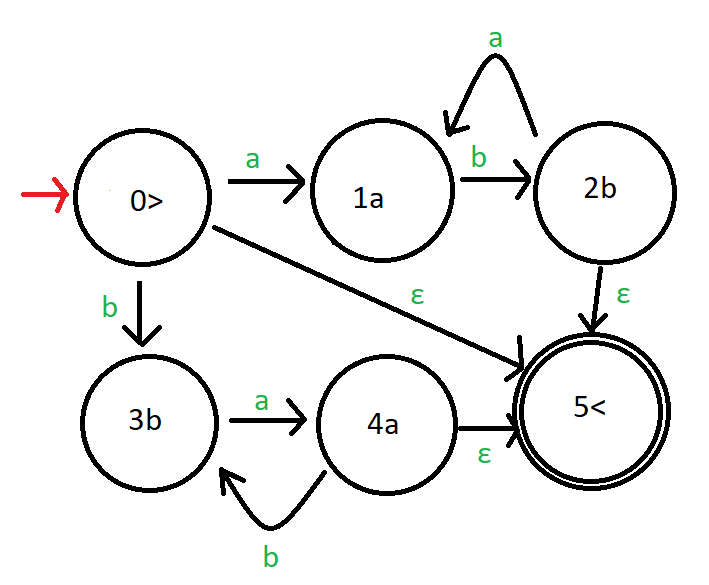
\includegraphics[scale=0.5]{06.png}

Это совпадает с автоматом, который предложен в описании, если определить эпсилон переход из вершины в отдельную.

Да, это регулярное выражение порождает язык, который принимает предложенный автомат, т.к. автомат, построенный на основании этого регулярного выражения совпадает с предложенным.

\subsection{Задача 5}

\textbf{1.}
$\mathcal{A}$ = (\{$q_0, q_1\}$, \{0, 1\}, $\delta$, $q_0$, $q_0$)

Состояние $q_0$ отвечает за четное число нулей, состояние $q_1$ отвечает за нечетно количество нулей. Соответсвенно буква 1 не меняет состояние автомата, а буква 0 переводит его в другое состояние. Функция $\delta$ задана графом.

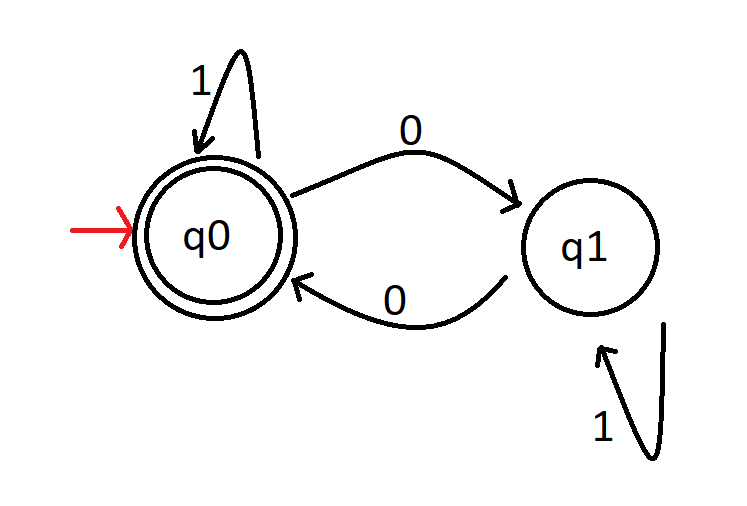
\includegraphics[scale=0.5]{03.png}
\newline
\textbf{2.}
$\mathcal{B}$ = (\{$q_0, q_1\}$, \{0, 1\}, $\delta$, $q_0$, $q_1$)

Состояние $q_0$ отвечает за четное число нулей, состояние $q_1$ отвечает за нечетно количество нулей. Соответсвенно буква 1 не меняет состояние автомата, а буква 0 переводит его в другое состояние. Функция $\delta$ задана графом.
Тут меняется только принимающее состояние.

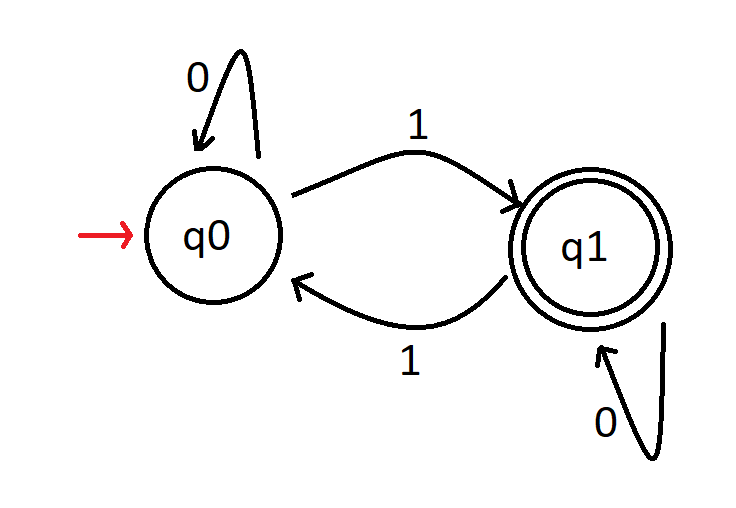
\includegraphics[scale=0.5]{04.png}
\newline
\textbf{3.}
$\mathcal{C}$ = (\{$q_0, q_1, q_2, q_3\}$, \{0, 1\}, $\delta$, $q_0$, $q_1$)
Состояние $q_0$ отвечает за четной количество единиц и нулей, состояние $q_2$ отвечает за нечетное количество нулей и четное количество единиц, состояние $q_3$ отвечает за нечетное количество нулей и единиц, состояние $q_1$ отвечает за четной количество нулей и нечетное количество единиц.
Принимающее состояние - $q_1$, как того требует условие. Все переходы из одного состояния автомата в другое следует из здравого смысла, а функция переходов представлена в виде графа.

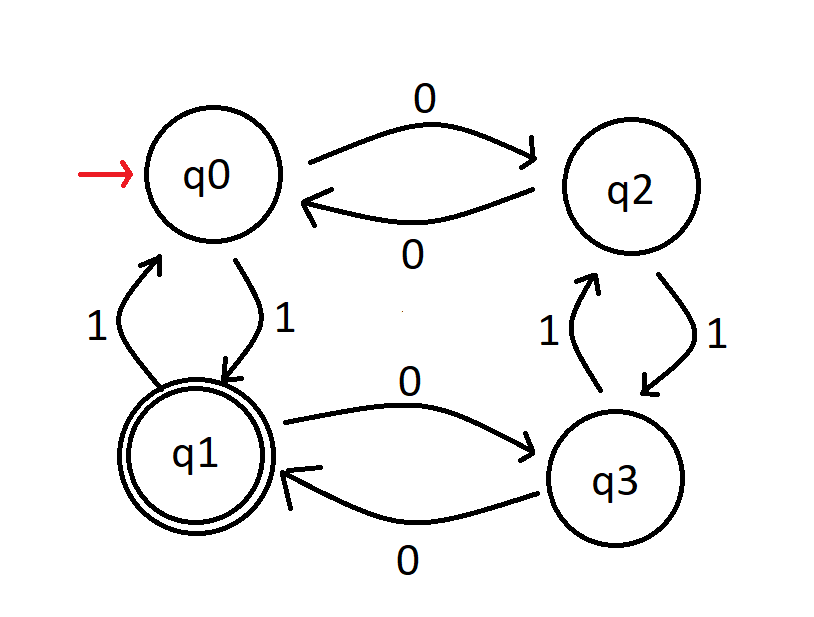
\includegraphics[scale=0.5]{05.png}


\end{document}